% Capítulo 4
\chapter{Fundamentação Teórica}\label{cap:fundamentacao-teorica}

Este capítulo está organizado para introduzir os conceitos-chave e explicar detalhadamente cada seção. Serão apresentados os fundamentos teóricos que sustentam o desenvolvimento e a aplicação de dois modelos fundamentais para a implementação da proposta: o modelo cognitivo e o modelo de template multicamadas para geração automática de questões. Cada subseção abordará os conceitos essenciais relacionados a esses modelos, detalhando suas características, funcionamento e contribuições para o objetivo final deste trabalho.

\section{Modelo Cognitivo}
A construção de questões em larga escala, por meio de processos automatizados, tem-se tornado uma prática cada vez mais relevante na área de avaliações educacionais. Nesse contexto, a elaboração de um modelo cognitivo sólido constitui um passo fundamental para embasar a Geração Automática de Questões (\gls{aig}). De modo geral, modelos cognitivos podem ser definidos como descrições explícitas de como os estudantes processam informações e resolvem tarefas específicas, envolvendo as habilidades e os raciocínios que se espera que demonstrem em uma dada questão. O processo de construção desse modelo, conforme discutido por \parencite{gierl2021}, esta técnica consiste em identificar, organizar e documentar de forma sistematizada os conceitos, parâmetros e restrições que caracterizam tanto a criação de uma questão quanto a forma como os estudantes são esperados a resolvê-la.

A relevância do modelo cognitivo fica  mais evidente quando se busca a replicabilidade e a qualidade das questões geradas. Esse detalhamento fornece a base para a elaboração dos templates, os quais orientam a criação de questões capazes de manter o mesmo nível de complexidade, exigência cognitiva e alinhamento ao conteúdo que se pretende avaliar. Dessa forma, o modelo cognitivo funciona como um roteiro que descreve tanto os conteúdos quanto a lógica da questão gerada.

O modelo cognitivo é a base fundamental para a criação dos templates, pois organiza e descreve todos os elementos necessários para sua construção. Os templates, por sua vez, atuam como estruturas que convertem essas informações de forma efetiva, resultando em questões de avaliação individual claras e alinhadas aos objetivos de ensino.


\section{Estrutura do Modelo Cognitivo}

O modelo cognitivo funciona como um guia para organizar os elementos necessários para a construção dos templates. Estes templates servem como estruturas que traduzem as diretrizes estabelecidas no modelo cognitivo em questões, claras, consistentes e alinhadas aos objetivos educacionais \parencite{keehner2017, gierl2017}. Para garantir a qualidade e replicabilidade, o modelo cognitivo deve ser estruturado de maneira a detalhar os seguintes aspectos fundamentais : 

\subsection{Problemas e Cenários}

A primeira etapa do processo de construção do modelo cognitivo consiste em definir claramente o objetivo da avaliação, identificando o problema central que servirá de base para elaboração dos cenários específicos. Em uma disciplina de algoritmos que aborda estruturas de repetição, podemos optar por explorar aspectos como o tipo de laço ou os componentes fundamentais de uma estrutura controlada por um contador. Dessa forma, podemos assegurar que as habilidades específicas a serem avaliadas estejam claramente refletidas na questão. E, posteriormente, elaborar possíveis cenários relacionados ao problema principal. Nas avaliações sobre estruturas de repetição, podemos incluir cenários que envolvam a identificação do tipo de laço utilizado em um trecho de código, a utilização de contadores para controlar iterações ou a aplicação de estruturas de repetição em situações práticas de desenvolvimento de algoritmos. Cada cenário amplia a diversidade das questões, mantendo a coerência com o objetivo da avaliação.

\subsection{Fontes de Informação}

As fontes de informação constituem o conjunto de conteúdos e matérias que podem abranger dados quantitativos, textos, fórmulas, diagramas, trechos de código, figuras ou qualquer outro elemento que possibilite aos estudantes acionar os conhecimentos e habilidades que se deseja avaliar. Cada fonte de informação deve ser descrita de forma detalhada, de modo a estabelecer claramente a relação entre o conteúdo apresentado e as características a serem avaliadas.


\subsection{Características (\textit{Features})}

As características (\textit{features}) são atributos fundamentais que compõem as dimensões ou variáveis do modelo cognitivo. Elas definem os aspectos que podem ser ajustados na criação dos templates. Na prática, cada característica é composta por três componentes principais: elementos, valores e restrições, descritos a seguir:

\begin{enumerate}
\item \textbf{Elementos} : Elementos representam as variações possíveis dentro de uma categoria ou dimensão específica da \textit{feature}, permitindo a manipulação do conteúdo através de componentes básicos que podem ser uma variável numérica, um trecho de código ou um termo técnico relevante para a questão. Os elementos devem ser construídos de forma a facilitar a combinação de um elemento com outro.

\item \textbf{Variáveis} : Valores são as possíveis combinações que os elementos podem assumir dentro de uma faixa de opções. Eles definem as variações quantitativas ou qualitativas que um elemento pode ter.

\item \textbf{Restrições} : Restrições são regras ou condições que limitam como os elementos e seus valores podem ser combinados. Elas garantem que as combinações resultantes sejam válidas, coerentes e alinhadas aos objetivos da questão, evitando a geração de questões inválidas ou sem sentido.

\end{enumerate}


A figura \ref{fig:cognitive-model} apresenta a estrutura hierárquica do modelo cognitivo para geração automática de questões, destacando os principais componentes e suas inter-relações. Ela organiza os elementos em três níveis principais : problemas e cenários, fontes de informação e características (\textit{features}). Essa visualização facilita o entendimento do processo de construção do modelo cognitivo.

\begin{figure}[ht]
	\centering
	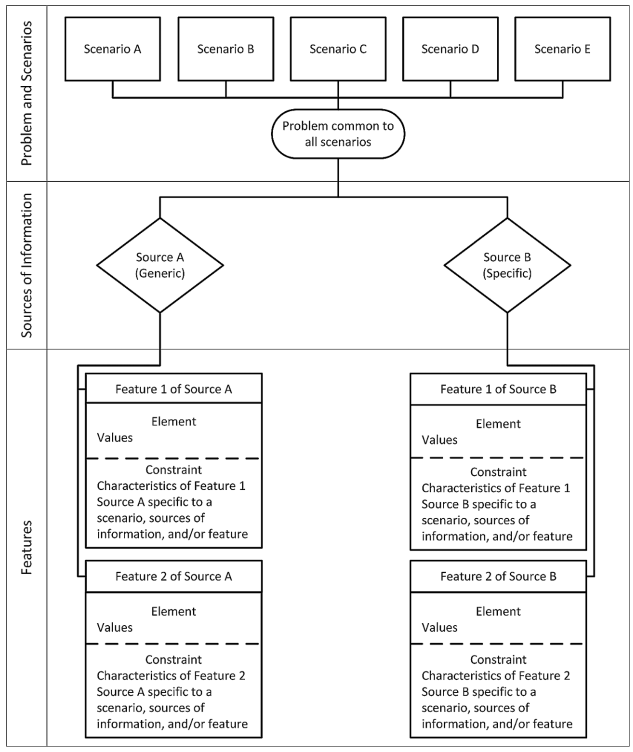
\includegraphics[width=16cm]{./imagens/capitulo4/cognitive-model}
	\caption{Estrutura do modelo cognitivo adaptado (\cite[p. 33]{gierl2021}.)}
	\label{fig:cognitive-model}
\end{figure}


\section{Relação do Modelo Cognitivo e a Construção dos Templates }

O modelo cognitivo é o fundamento para a construção dos templates, pois organiza e descreve todos os conceitos, regras, parâmetros, limites e relações necessárias para a construção das questões. Os templates, por sua vez, convertem o modelo cognitivo em estruturas para gerar diferentes versões de questões, sendo assim a relação entre o modelo cognitivo e os templates pode ser resumida nos seguintes pontos:


\begin{enumerate} \item \textbf{Definição de elementos básicos de uma questão:} O modelo cognitivo descreve quais componentes  precisam estar presentes para que a questão seja relevante e alinhado aos objetivos de aprendizado. O \textit{template} organiza esses componentes em uma estrutura pronta para gerar diferentes versões de questão \parencite{lane2016}.

\item \textbf{Combinação e manipulação de parâmetros:}
Enquanto o modelo cognitivo define as regras de como os conteúdos e as habilidades podem ser combinados, o \textit{template} coloca essas regras em prática. Integra os diversos elementos para criar questões com diferentes níveis de complexidade, mantendo a coerência com a proposta original \parencite{embretson2017}.

\item \textbf{Padronização e escalabilidade:}
A adoção de um modelo cognitivo bem elaborado facilita a padronização do processo de elaboração de questões em grande escala. Como os \textit{templates} seguem o mesmo conjunto de regras e estruturas, as questões criadas tendem a manter consistência em termos de conteúdo, formato e nível de exigência cognitiva \parencite{gierl2017}.

\item \textbf{Validação e ajustes contínuos:}
Se um \textit{template} gerar uma questão que se revele incoerente ou sem lógica, é possível identificar rapidamente se o problema está no modelo cognitivo ou no próprio \textit{template}, permitindo o ajuste da regra que originou a inconsistência. Dessa forma, a correção ocorre em nível conceitual (no modelo) ou na estrutura do \textit{template}, preservando a qualidade das questões e mantendo-os alinhados aos propósitos da avaliação \parencite{gierlbulutzhang2018}.
\end{enumerate}


\section{Templates Multicamadas}

Modelos de templates multicamadas são estruturas utilizadas para gerar questões automaticamente com base em variações sistemáticas de componentes dentro de um template. A construção desses modelos pode seguir diferentes níveis de complexidade — como os modelos de 1 camada (\textit{1-layer}), 2 camadas (\textit{2-layers}) ou múltiplas camadas (\textit{n-layers}) — dependendo de quantas camadas de abstração e variação são incorporadas. A ideia central é permitir que, a partir de um único modelo, seja possível gerar um grande número de questões com diferentes combinações de conteúdo, mantendo a estrutura lógica do modelo . 

\subsection{Modelos de Template de uma camada \textit{(1-Layer)}}

Segundo \parencite{gierl2021}, um modelo de questão pode ser definido como um template que especifica os componentes manipuláveis de uma questão, e cada componente carrega um valor ou um intervalo de valores que podem ser alterados de forma sistemática para gerar novas questões . O modelo de questão de 1-layer ("template de camada única") constitui uma abordagem na qual se manipulam apenas alguns elementos dentro de uma estrutura fixa para produzir novas questões. Este modelo é estruturado por um único template, onde cada elemento pode assumir diferentes valores previamente estabelecido \parencite{lai2013}. A seguir será apresentado as principais características desse template de uma camada e posteriormente o template multicamadas, sua forma, aplicações práticas e limitações.

\subsection{Estrutura do Modelo}

O modelo de template (\textit{1-layer}) parte de um modelo cognitivo ou uma questão já existente com ponto de partida para identificar os elementos manipuláveis, e em seguida é isolado os elementos variáveis da questão como números, termos, contextos que podem assumir diversas variações. Este modelo inclui : 

\begin{itemize}
    \item \textbf{Enunciado (\textit{Stem})} : Texto que apresenta a pergunta ou situação-problema
    \item \textbf{Elementos (\textit{Features})} : Constitui cada parte que pode mudar dentro do texto, todos os elementos estão em um só nível, compondo o corpo da questão. Esses elementos podem ser textos ou valores numéricos, em que cada elemento terá um intervalo ou conjunto de valores permitidos.
\end{itemize}

\section{Fluxo para templates de uma camada (\textit{1-Layer})}

O processo de geração de templates de \textit{uma camada} (\textit{1-Layer})  é composto por três etapas principais: (1) construção do modelo cognitivo, (2) definição do modelo de template, e (3) geração das questões. Cada uma dessas etapas será detalhada nas seções seguintes. 

\subsection{Etapa 1 - Modelo Cognitivo }

Para construir o modelo cognitivo, é necessário identificar os \textbf{cenários} e \textbf{problemas} a serem tratados, as \textbf{fontes de informação} envolvidas, as \textbf{características} e \textbf{restrições} que devem ser seguidas. A partir dessa estrutura, podemos descrever a lógica que rege o comportamento do template. A Figura \ref{fig:condicional-simples}  apresenta um exemplo de modelo cognitivo de uma camada (\textit{1-layer}), baseado em problemas de introdução à programação que envolve condicional simples.  A partir da construção do modelo cognitivo podemos produzir um ou mais templates baseado nesta estrutura. Esses templates seguirão os mesmos princípios definidos pelo modelo, respeitando suas características, limites e restrições para garantir a coerência no desenvolvimento do template.  O passo seguinte é a construção do template em si, tornando como base o modelo apresentado, o objetivo é transformar a lógica apresentada graficamente em estruturas de templates reutilizáveis que podem ser aplicadas em diferentes contextos. 
\begin{figure}[ht]
	\centering
	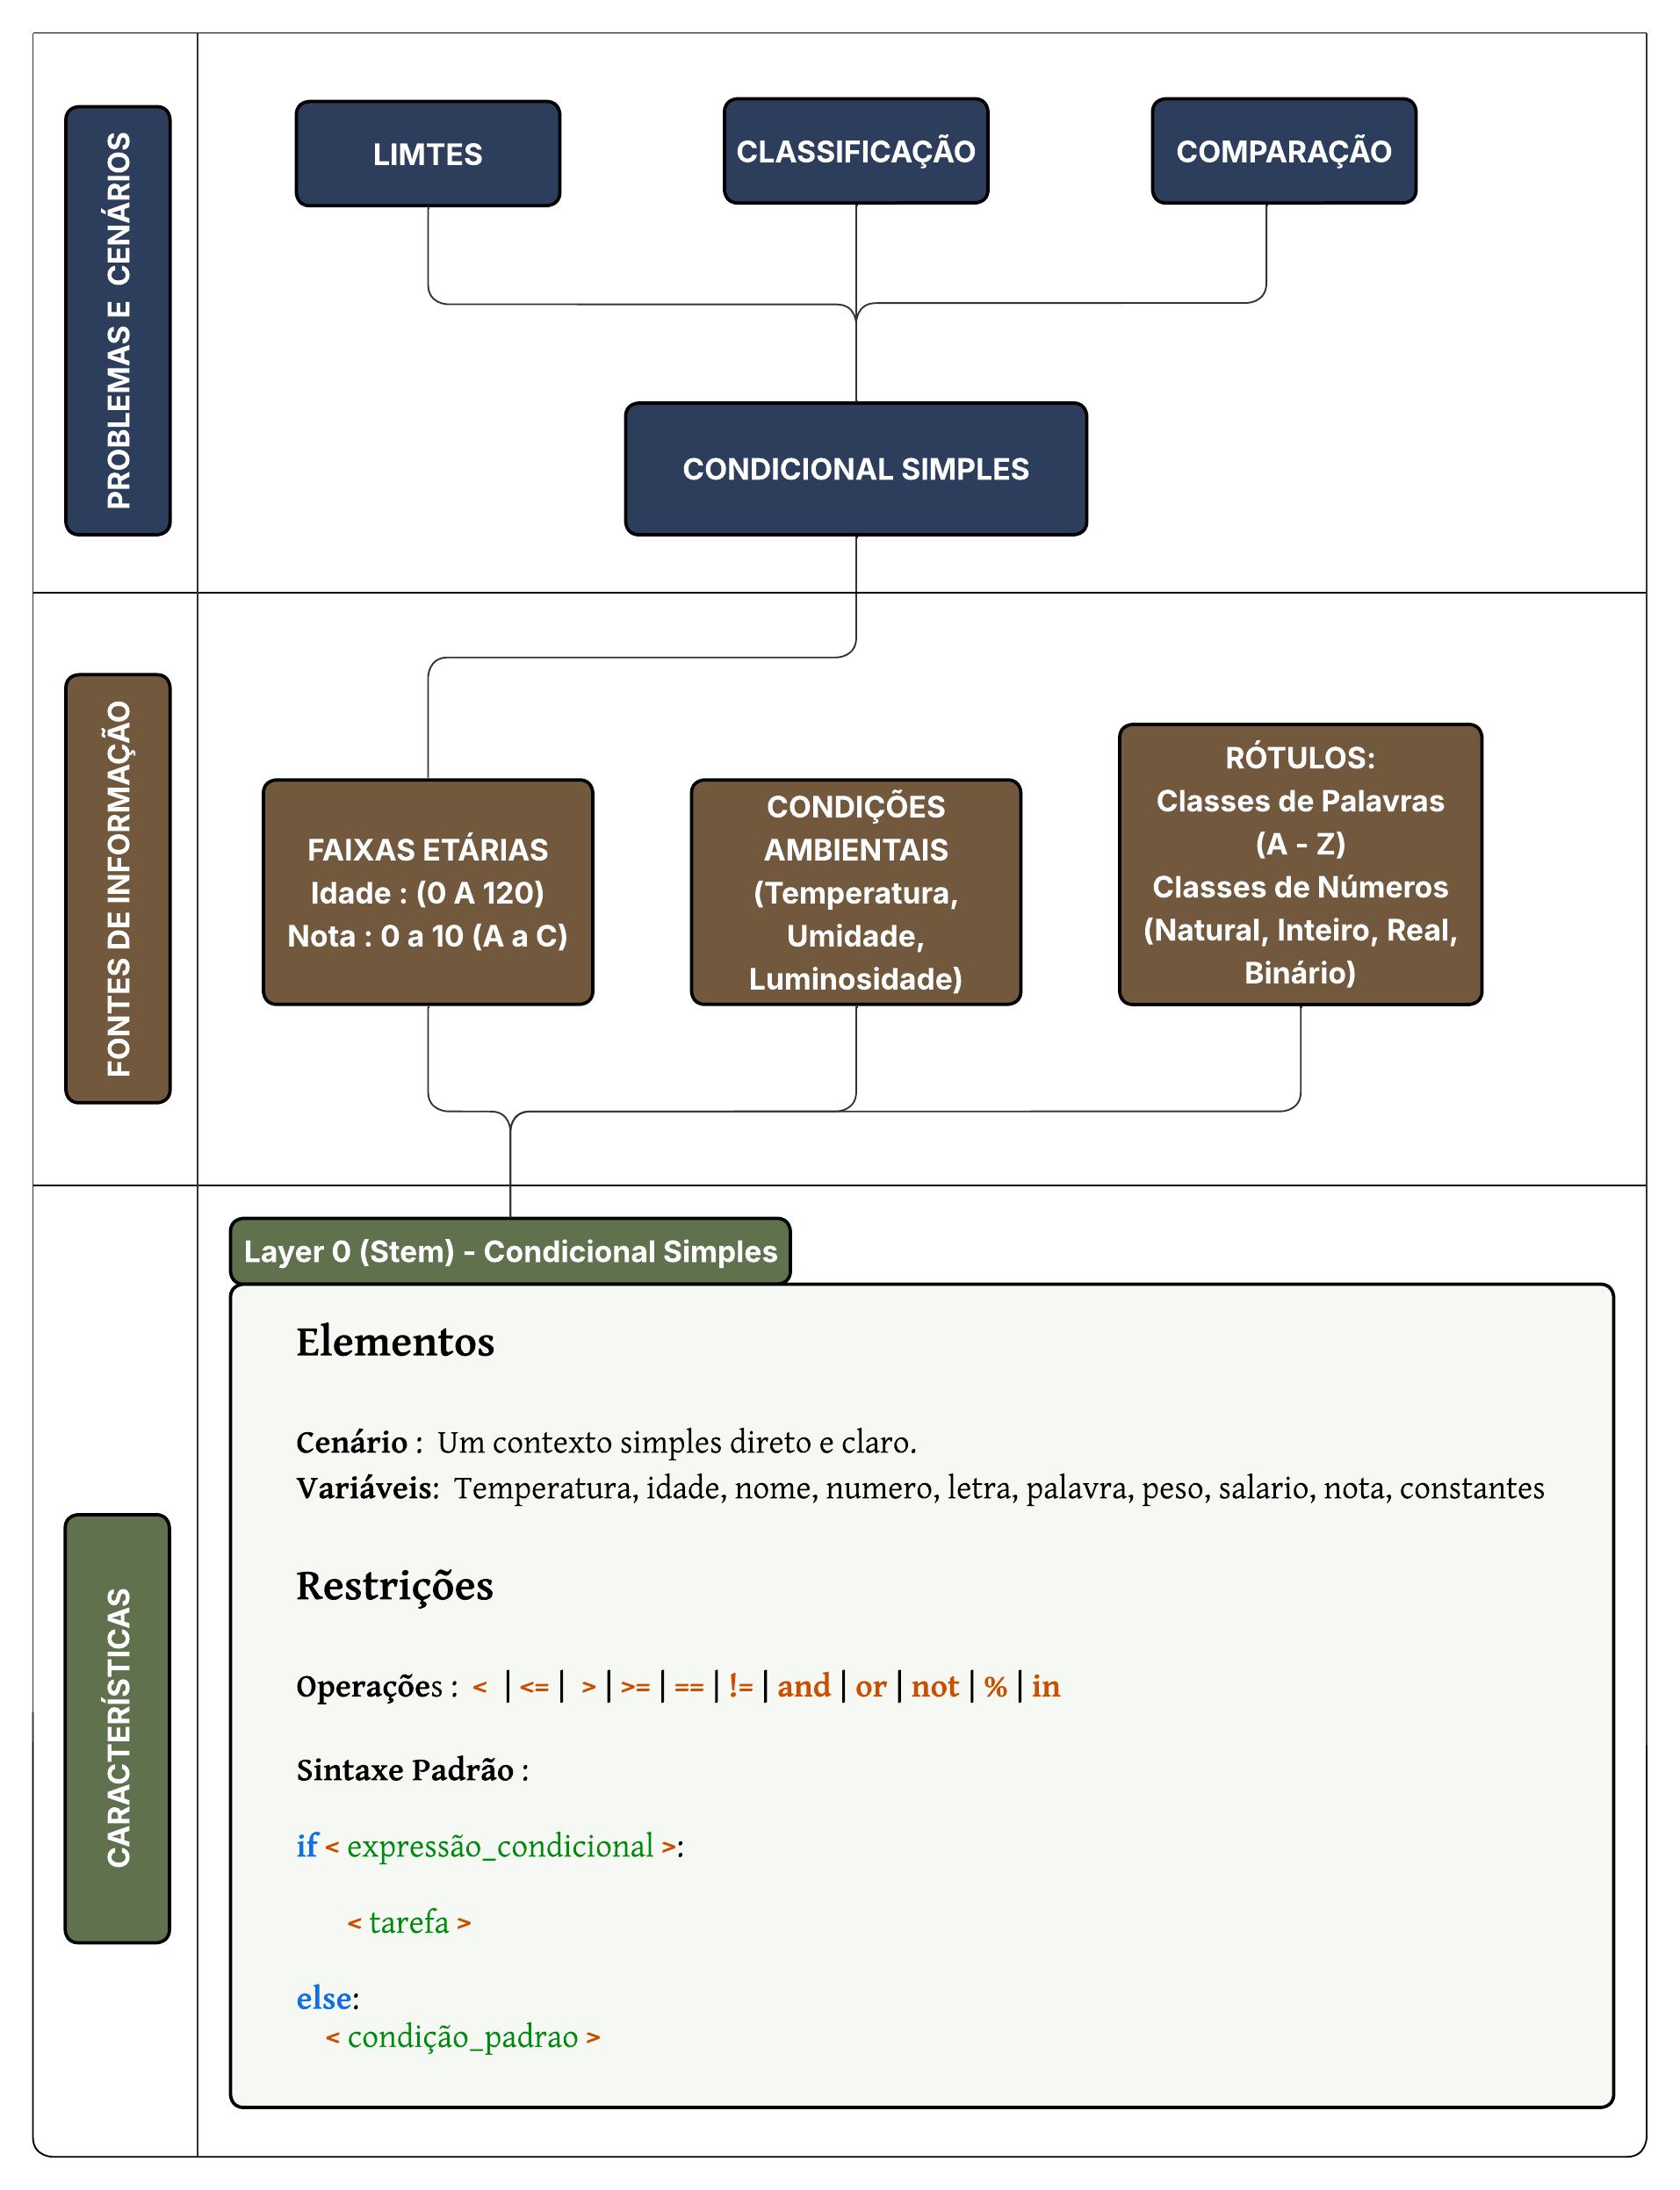
\includegraphics[width=16cm]{./imagens/capitulo4/modelo-cognitivo-1-layer}
	\caption{Modelo Congitivo : Condicional Simples  (Autoria própria, 2025)}
	\label{fig:condicional-simples}
\end{figure}
\subsection{Etapa 2 - Construção do template} 

A Tabela \ref{tab:template-questoes-elementos} demonstra como a questão de referência baseado no modelo cognitivo se relaciona com o template e os respectivos elementos que podem variar. Na primeira linha, “\textbf{Questão de Referência}”, contém o enunciado-base que exemplifica o problema a ser resolvido. Na segunda linha, “\textbf{Template (\textit{Stem})}”, temos a estrutura geral do enunciado, com espaços reservados para a inserção de diferentes conteúdos possíveis, podendo ainda incluir textos fixos que complementam o enunciado.

\begin{table}[htbp]
\centering
\begin{tabular}{|l|p{10cm}|}
\hline
\textbf{Questão de Referência} 
& 
Um sistema digital classifica o tipo de acesso dos usuários com base em seu perfil. Escreva um programa que leia o tipo de usuário, utilizando \texttt{if-else}, exiba a permissão correspondente:

\begin{tabular}{|l|l|}
    \hline
    \textbf{Usuario} & \textbf{Permissão} \\
    \hline
    Visitante & Acesso Limitado \\
    Comum & Acesso Parcial \\
    Premium & Acesso Completo \\
    \hline
  \end{tabular}

Mostre na tela qual é o tipo de acesso liberado para o usuário informado.
\\
\hline

\textbf{Template (\textit{Stem})} 
& \texttt{\{contexto-geral\} \{contexto-específico\} \{tabela-condicional\} \{solicitação\}} 
\\
\hline

\textbf{Elementos (Variáveis)} 
& 
\textbf{contexto-geral:}
\begin{itemize}
  \item[{[ 0 ]}] Um sistema digital é responsável por tomar decisões automáticas com base nos dados dos usuários. 
  \item[{[ 1 ]}] Uma plataforma de atendimento inteligente analisa o perfil dos usuários para oferecer respostas personalizadas.  
\end{itemize}

\textbf{contexto-específico:}
\begin{itemize}
  \item[{[ 1 ]}] O sistema considera o tipo de usuário cadastrado para determinar permissões de acesso. 
  \item[{[ 0 ]}] A plataforma verifica a quantidade de interações feitas por semana e o tempo médio de resposta dos usuários. 
\end{itemize}

\textbf{tabela-condicional:}
\begin{itemize}
  \item[{[ 0 ]}]
  \begin{tabular}{|l|l|}
    \hline
    \textbf{Tipo de usuário} & \textbf{Permissão} \\
    \hline
    Visitante & Acesso restrito \\
    Comum & Acesso moderado \\
    Premium & Acesso total \\
    \hline
  \end{tabular}

  \item[{[ 1 ]}]
  \begin{tabular}{|l|l|}
    \hline
    \textbf{Interações semanais} & \textbf{Classificação} \\
    \hline
    $\geq 5$ & Ativo \\
    $< 5$ & Inativo \\
    \hline
  \end{tabular}
\end{itemize}

\textbf{solicitação:}
\begin{itemize}
  \item[{[ 0 ]}] Crie uma estrutura \verb|if-else| que avalie as condições apresentadas e exiba o resultado. 
  \item[{[ 1 ]}] Desenvolva um algoritmo que, com base nas variáveis, aplique as regras corretamente. 
\end{itemize}
\\
\hline
\end{tabular}
\caption{Template de questões (Elaboração Própria, 2025)}
\label{tab:template-questoes-elementos}
\end{table}


\subsection{Etapa 3 - Geração das questões}

No modelo de uma camada (\textit{1-Layer}), a geração de questões ocorre por meio da manipulação de um número limitado de elementos em um único nível. Essa abordagem é relativamente simples e de fácil implementação, pois se baseia em poucas variáveis para a criação das novas questões. Em razão dessa simplicidade, as variações ocorrem de forma linear, fazendo com que a diversidade das questões geradas seja menor. Ainda assim, este modelo é bastante útil quando se deseja alterar minimamente o contexto ou a a formulação geral, embora, por este mesmo motivo faz com que os estudantes percebam com mais facilidade padrões ou similaridades entre as questões geradas. 
Como ilustra a Tabela \ref{tab:questoes-geradas}, cada elemento variável é manipulado em um único nível, modificando apenas os índices dos itens pontuais tais como: contexto geral, contexto específico e solicitação para a geração de novas questões. Essa estrutura mais enxuta favorece a compreensão das etapas de modelagem, sendo indicada especialmente para professores que estão em fase de aprendizado na construção de \textit{templates}. Nesse sentido, o modelo \textit{1-layer} funciona como uma base inicial, antes de se evoluir para modelos mais complexos que exigem a manipulação de múltiplos níveis, como ocorre nos templates multicamadas (\textit{n-layers}) que será discutido na próxima seção.



\begin{table}[H]
    \centering
    \begin{tabular}{|p{14cm}|}
        \hline
        \textbf{Questões Geradas} \\ 
        \hline
        \\
        \textbf{Questão 1:} Um serviço de streaming define a qualidade de reprodução de vídeo com base no plano contratado pelo usuário. A quantidade de dispositivos conectados simultaneamente determina a resolução disponível para reprodução:
        \vspace{1em}
        
    
        
        \begin{minipage}{\linewidth}
        \centering
        \begin{tabular}{|c|c|}
                \hline
                \textbf{Dispositivos} & \textbf{Qualidade} \\
                \hline
                1 & 4K \\
                \hline
                2--3 & FullHD \\
                \hline
                > 3 & HD \\
                \hline
        \end{tabular}

    \end{minipage}

        \vspace{1em}

        Desenvolva um algoritmo que leia o número inteiro conforme a tabela e utilize uma estrutura if-else para imprimir a qualidade de vídeo liberada.\\[1em]
        \\
        \textbf{Questão 2:} Um sistema digital é responsável por tomar decisões automáticas com base nos dados dos usuários. Escreva um programa que leia o tipo de usuário, e classifique o tipo de acesso dos usuários com base em seu perfil:
        \vspace{1em}
        
    
        
        \begin{minipage}{\linewidth}
        \centering
        \begin{tabular}{|c|c|}
                \hline
                \textbf{Usuário} & \textbf{Permissão} \\
                \hline
                Visitante & Acesso Limitado \\
                \hline
                Comum & Acesso Parcial \\
                \hline
                Premium & Acesso Completo \\
                \hline
        \end{tabular}

    \end{minipage}

        \vspace{1em}

        Mostre na tela qual é o tipo de acesso liberado para o usuário informado.\\[1em]
        \\
        \textbf{Questão 3:} Alguns aplicativos utilizam várias estratégias para adaptar a experiência conforme as condições de uso. Em um aplicativo para dispositivos móveis, a qualidade de transmissão é ajustada automaticamente com base no plano de dados do usuário:.
        \vspace{1em}
        
    
        
        \begin{minipage}{\linewidth}
        \centering
        \begin{tabular}{|c|c|}
                \hline
                \textbf{Consumo Diário (em GB)} & \textbf{Qualidade de Vídeo} \\
                \hline
                1 & Alta (4K) \\
                \hline
                2--3 & Média (FullHD) \\
                \hline
                > 3 & Baixa (HD) \\
                \hline
        \end{tabular}

    \end{minipage}

        \vspace{1em}

        Desenvolva um programa que leia o consumo diário de dados móveis e informe a qualidade de vídeo correspondente, utilizando estruturas \texttt{if-else}.\\[1em]
        \\
      
        \hline
    \end{tabular}
    \caption{Questões geradas (Elaboração própria, 2025)}
    \label{tab:questoes-geradas}
\end{table}




  

\section{Fluxo para templates multicamadas (n-Layers)}

A abordagem de multicamadas (\textit{n-layers}) amplia consideravelmente a capacidade de variações e a complexidade na geração de questões quando comparada ao modelo de camada única (\textit{1-layer}).  Enquanto que no modelo de uma camada é manipulado um pequeno conjunto de elementos em um \textit{template}, no modelo (\textit{n-layer}) cada camada adiciona uma nova estrutura de \textit{sub-templates} que possibilita combinar múltiplas estruturas de templates organizadas em níveis hierárquicos. Dessa forma, passa a ser viável embutir os elementos, criando estruturas cada vez mais complexas que resultam em uma variedade maior  de questões geradas conforme a proposta de  \parencite{lai2013}. No entanto, essa maior diversidade traz também um aumento na complexidade de construção, pois a construção de modelos em múltiplas camadas requer planejamento adicional, tempo para projetar, validar e revisar cada camada e, principalmente a experiência de quem elabora as questões \parencite{gierl2021}.  

\subsection{Etapa 1 - Modelo de Template Multicamadas }

O fluxo de elaboração do template multicamadas mantém‐se idêntico ao do modelo de camada única, a principal diferença é a possibilidade de adicionar \textit{sub-templates} dentro do template principal que agrupam blocos adicionais de informações. Cada nova camada introduz cenários e variáveis extra, ampliando significativamente o conjunto de questões geradas. Para ilustrar na prática, considere um problema geral de programação cujo menu apresenta quatro opções (A, B, C e D). As três primeiras são \textit{sub-templates} de dificuldade crescente - fácil, moderada e difícil, enquanto que a quarta finaliza o programa. Assim, há uma camada principal que exibe o menu e as camadas secundárias que detalham as operações específicas de cada opção. As Figuras \textbackslash{}ref\{fig:template-1\} e \textbackslash{}ref\{fig:template-2\} apresentam o modelo desse problema sob a abordagem multicamadas. O \textbackslash{}textit\{stem\} (camada raiz) simula a interface de uma calculadora; colchetes simples delimitam pontos de variação, ao passo que colchetes duplos indicam a substituição por um sub-template definido na camada subsequente. Cada índice numérico em listas internas corresponde a um valor possível assumido pelo template, permitindo reutilizar a estrutura original sem comprometer a coerência da questão. Dessa forma, o modelo favorece tanto a escalabilidade quanto o controle de dificuldade, preservando a integridade conceitual da questão gerada.

\begin{figure}
    \centering
    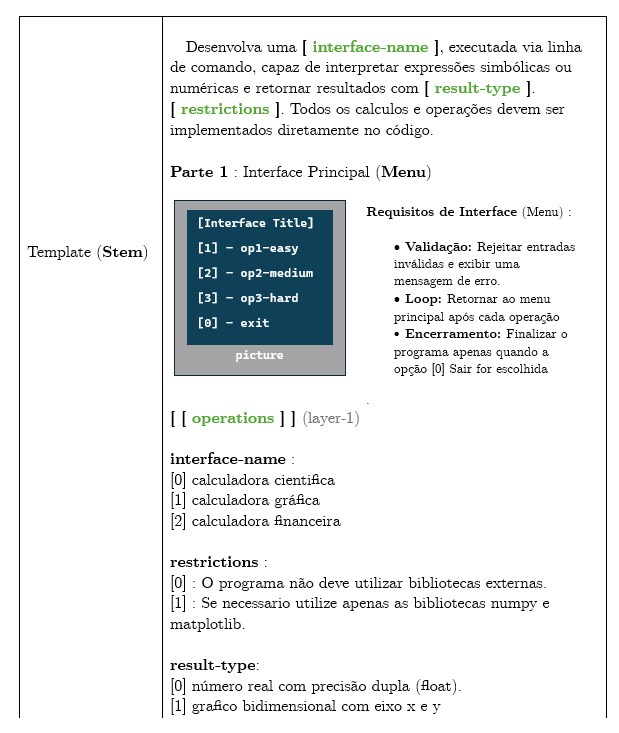
\includegraphics[width=12cm]{./imagens/capitulo4/template-1.png}
    \caption{Template calculadora parte 1 - (Autoria própria, 2025)}
    \label{fig:template-1}
\end{figure}

\begin{figure}
    \centering
    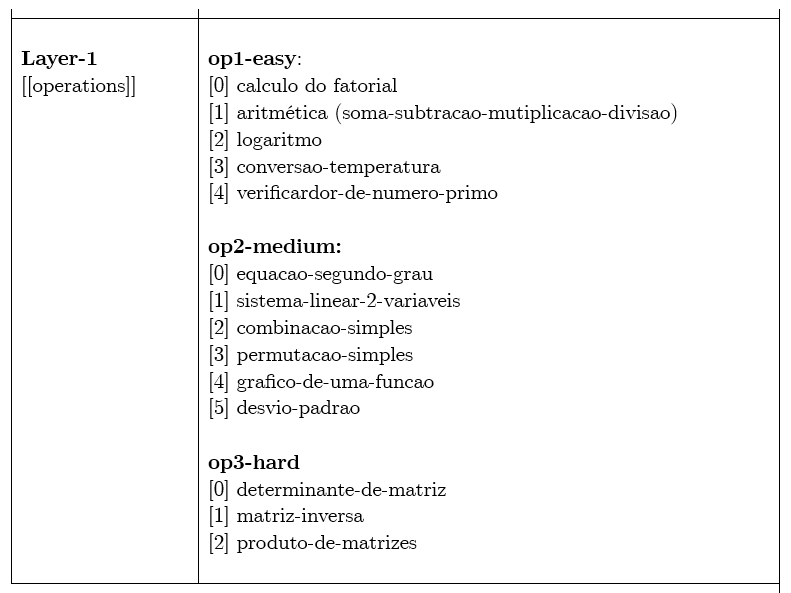
\includegraphics[width=12cm]{./imagens/capitulo4/template-2.png}
    \caption{Template calculadora parte 2 - (Autoria própria, 2025)}
    \label{fig:template-2}
\end{figure}


--------------  Questões geradas -----------
Considere a questão gerada ilustrada nas Figuras \ref{fig:questao-referencia-part-1} e \ref{fig:questao-referencia-part-2}. A primeira parte descreve um menu de calculadora; a segunda detalha três categorias de operações (fácil, moderado, e difícil), baseado no modelo multicamadas é possível substituir o contexto de “calculadora” por múltiplos cenários similares a um menu, como por exemplo, interface de computador, caixa eletrônico, jogo simples, painel de controle industrial, tudo isso sem alterar estrutura e a lógica de dificuldade da questão. Se, para cada nível de dificuldade, forem especificadas 20 variações e adotarmos apenas um cenário, já obtemos 20×20×20=8.000 variações. Com dois ou três cenários, esse quantitativo pode alcançar 16.000 ou 24.000 variações respectivamente, demonstrando o poder combinatório deste modelo.


\begin{figure}[ht]
	\centering
	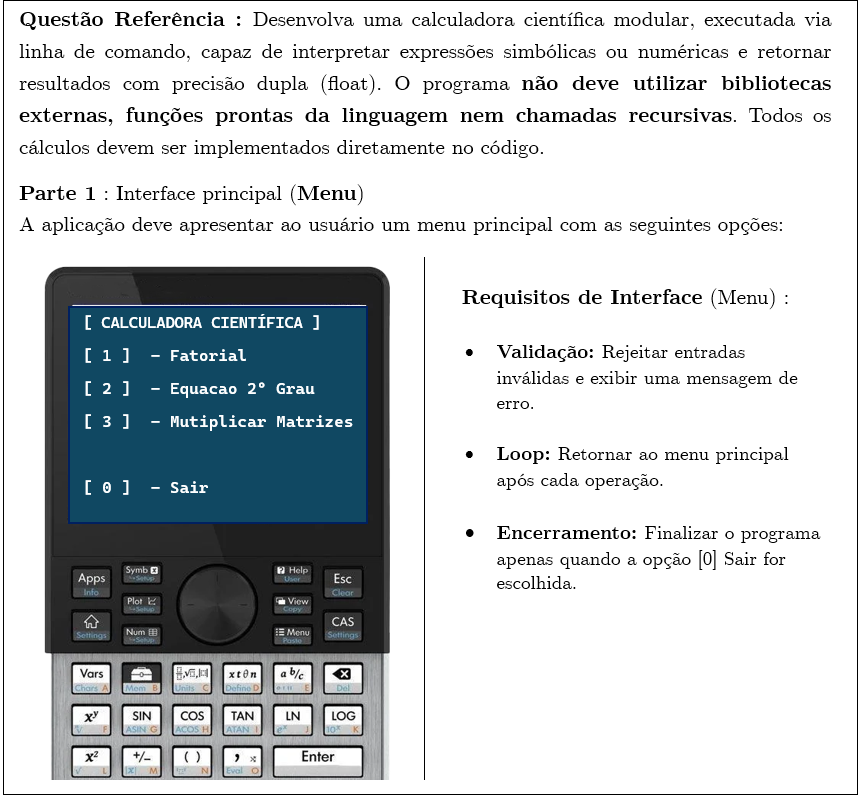
\includegraphics[width=12cm]{./imagens/capitulo4/questao-referencia-1.png}
	\caption{Questão de referência - parte 1 (Autoria própria, 2025)}
	\label{fig:questao-referencia-part-1}
\end{figure}


\begin{figure}[ht]
    \centering
    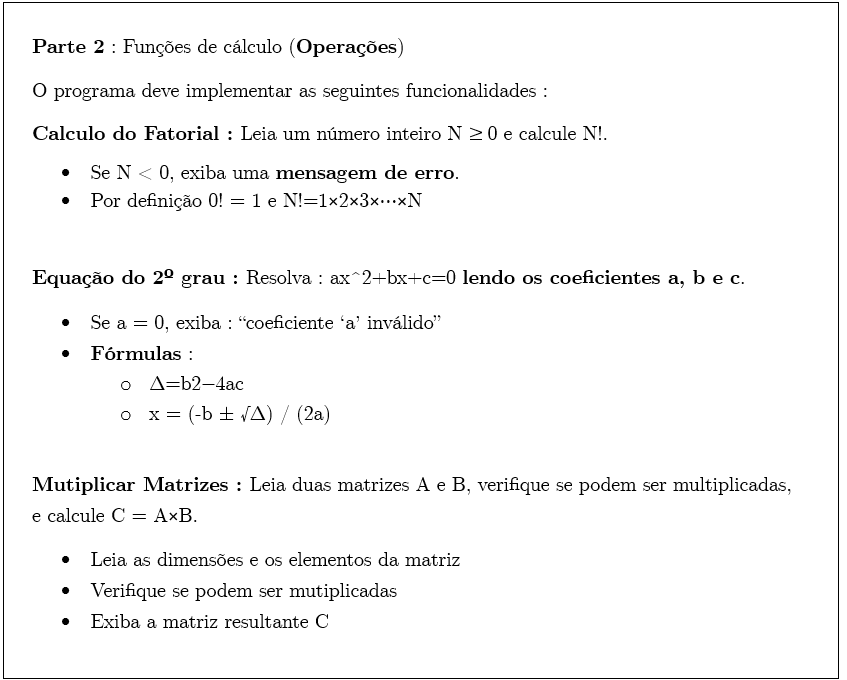
\includegraphics[width=12cm]{./imagens/capitulo4/questao-referencia-2.png}
    \caption{Questão de referência parte 2 - (Autoria própria, 2025)}
    \label{fig:questao-referencia-part-2}
\end{figure}


\subsection{Razões para utilizar templates na geração de questões}

A geração automática de questões baseada em \textit{templates} é hoje uma estratégia versátil e operacionalmente viável para gerar questões em escala. A adoção de estruturas pré-definidas garante padronização, controle de complexidade e rastreamento dos erros, além de não exigir muitos recursos computacionais quando comparado com as abordagens que não utilizam templates. Essas abordagens dependem de uma grande bases de dados e de modelos extensivamente treinados, que resulta em sua maioria, questões menos complexas, com criatividade limitada e com qualidade variável. Além disso, conforme \parencite{maity2024} menciona que, sistemas de geração automática de questões  baseadas em \gls{llm} tendem a gerar questões redundantes, enfrentam dificuldades na elaboração de problemas complexos, apresentam variação na qualidade das perguntas geradas e ainda estão sujeitos a riscos relacionados a vieses linguísticos. Estes fatores reforçam a atual preferencia pelo uso de \textit{templates} na geração automática de questões.

Em resposta à \textbf{(QP1)}, este trabalho adota o modelo de \textit{templates} multicamadas porque, além de preservar a clareza estrutural, acrescenta dois benefícios essenciais: (i) maior poder combinatório, viabilizando um conjunto mais amplo de questões, e (ii) representação hierárquica de cenários. Questões simples podem de fato, ser contempladas por um template de uma camada, entretanto problemas de programação que envolvem múltiplos cenários requerem uma arquitetura que reflita tal complexidade de forma reutilizável.

Quanto ao papel opcional do modelo cognitivo, a literatura recomenda que o professor o especifique este modelo sempre antes de desenvolver os templates \parencite{gierl2021}. No entanto, para questões fáceis ou moderadas, o custo adicional de elaborar um modelo cognitivo completo pode sobrepor seus benefícios. Por tanto neste trabalho, essa elaboração é opcional, ficando a cargo do autor do \textit{template} desenvolver ou não.

As discussões deste capítulo fundamentam o uso de templates, destacando sua mecânica e vantagens frente às abordagens com \gls{llm}. No capítulo seguinte, esses conceitos serão aplicados na prática, com a definição das estruturas que operacionalizam os templates multicamadas.



